\PassOptionsToPackage{dvipsnames}{xcolor}
\documentclass[a4paper,11pt]{report} %article

\usepackage{graphicx,subfigure,afterpage,hyperref,xspace,xcolor,caption,soul,geometry,pdfpages,stackengine,eso-pic,fancyhdr,hyphenat,listings,longtable,url,enumitem,fancyvrb,textcomp,eurosym,pbox}


%\usepackage[utf8]{inputenc} %to make the single quote appear correct after the encoding inserted above!

%command to substitute "{\em MyTaxyService}" with "\mts"
\newcommand{\mts}{\mbox{\normalfont\itshape myTaxiService}}
\geometry{margin=1in}

%header & footer style
\fancyhead{}
\fancyhead[C]{\iffloatpage{}{\slshape\rightmark}}
\fancyfoot{}
\fancyfoot[C]{\iffloatpage{}{\thepage}}
\renewcommand{\headrulewidth}{\iffloatpage{0pt}{0.4pt}}
\renewcommand{\footrulewidth}{\iffloatpage{0pt}{0.4pt}}
\pagestyle{fancy}
\renewcommand{\sectionmark}[1]{\markright{\thesection.\ #1}}
\renewcommand{\subsectionmark}[1]{\markright{\thesubsection.\ #1}}

%tOC style: sections bold 
\usepackage[subfigure]{tocloft}
\renewcommand{\cftsecfont}{\bfseries}
\renewcommand{\cftsecpagefont}{\normalfont\bfseries}% page numbers in bold
\renewcommand{\cftdotsep}{1}
\renewcommand{\cftsecleader}{\bfseries\cftdotfill{\cftsecdotsep}}% dot leaders in bold

%to keep the links of the TOC invisible
\hypersetup{
	colorlinks,
	citecolor=black,
	filecolor=black,
	linkcolor=black,
	urlcolor=black
}


\title{Politecnico di Milano\\A.A. 2015/2016\\Software Engineering 2\\ \bigskip 
Assignment 5: Project Plan\\
{\normalsize Version 1.0}}
\author{Alessandro Baldassari (mat. 841561) \\ Alberto Bendin (mat. 841734) \\ Francesco Giarola (mat. 840554)}


%to set the nested bullet lists style
\renewcommand{\labelitemii}{$\circ$}
%\renewcommand{\labelitemii}{}
\renewcommand{\labelitemiii}{$\diamond$}

%to avoid the hyphenation of the name of the software
\hyphenation{myTaxyService}

\begin{document}
	
	%fIRSTPAGE
	
	%pOLIMI-LOGO
	\begin{figure}[t]
		\centering
		\includegraphics[width=1\linewidth]{"Pictures/polimi-logo"}
		\label{fig:polimi-logo}
	\end{figure}
	
	\maketitle
		
	
	%bLANK-PAGE
	\thispagestyle{empty}
	\clearpage\mbox{}\clearpage

	
	
	
	%to number the section from 1 instead of 0.1 with the report class, without using the article class. Avoid the forced use of chapters to number from 1. Tailored for REPORT class!!!
	\renewcommand*\thesection{\arabic{section}}
	\renewcommand*\thesubsection{\arabic{section}.\arabic{subsection}}
	\renewcommand*\thesubsubsection{%
	\arabic{section}.\arabic{subsection}.\arabic{subsubsection}%
	}
	\setcounter{secnumdepth}{4}
	\setcounter{tocdepth}{4}
	

	
	%to change the page numbering from roman in the toc to arabic
	\pagenumbering{roman}
	\tableofcontents
	\newpage
	\pagenumbering{arabic}
	
	
	%to insert the writing "Page" above page numbers in the TOC
	\addtocontents{toc}{~\hfill\textrm{Page}\par}
	
	%tables style
	\renewcommand{\arraystretch}{1.2}
	\setlength{\tabcolsep}{12pt}
	
	\section{Introduction} 
		\subsection{Purpose and Scope}
			The main purpose of the project plan is to plan time, cost and resources adequately to estimate the work needed and to effectively manage risk during project execution. A failure to adequately plan reduces the project's chances of successfully accomplishing its goals.\smallskip\\
			Project planning generally consists of:
			\begin{itemize}
				\item Identifying deliverables and creating the work breakdown structure;
				\item Identifying the activities needed to complete those deliverables and networking the activities in their logical sequence;
				\item Estimating the resource requirements for the activities;
				\item Estimating time and cost for activities;
				\item Developing the schedule;
				\item Developing the budget;
				\item Resource allocation (organization of work loads);
				\item Risk planning.
			\end{itemize} 
			This document is based on an analysis made with two different algorithmic metrics of the system for \mts{}. The first one is the Function Points (FP), which is used to estimate the software dimension (code size), which is directly used to evaluate the cost. The second is the COCOMO II that is used to estimate the efforts required in the development of a project by taking in account: characteristics of people, products and process. 
			
		\subsection{List of Definitions and Abbreviations}
			The following acronyms are used in this document:
			\begin{itemize}
				\item FP: Function Points
				\item COCOMO: COnstructive COst MOdel
				\item ILF: Internal Logic File
				\item EIF: External Interface File
				\item PM: Person-Months
				\item SLOC: Source Lines of Code
				\item KSLOC: Thousands of SLOC
				\item SD: Scale Drivers
				\item EAF: Effort Adjustment Factor
				\item GUI: Graphical User Interface
			\end{itemize}
			The following definitions are used in this document:
			\begin{itemize}
				\item Deliverables: are work that are delivered to the customer, e.g. a requirement document for the system.
			\end{itemize}
	
	\pagebreak		
	\section{Function Point analysis}
		\subsection{Introduction}
			The Function Point estimation approach is based on the amount of functionalities in a software and their complexity. Indeed the effort to develop a software project grows with the number of external inputs and outputs, user interactions, files and interfaces used by the system; therefore a weight is associated to all these functionalities and the total effort is computed summing all the partial values.\bigskip \\
			The parameters used to perform this estimation are summarized in the following tables, taken from COCOMO II, Model Definition Manual at:\smallskip\\ \href{http://csse.usc.edu/csse/research/COCOMOII/cocomo2000.0/CII\_modelman2000.0.pdf}{http://csse.usc.edu/csse/research/COCOMOII/cocomo2000.0/CII\_modelman2000.0.pdf.}\bigskip\\
%			This first schema is used to determine the complexity-level function counts. It classifies each functionality into Low, Average and High complexity levels.\smallskip\\
%			\begin{minipage}{\linewidth}
%				%			\vspace*{-0.35cm}
%				\makebox[\linewidth]{
%					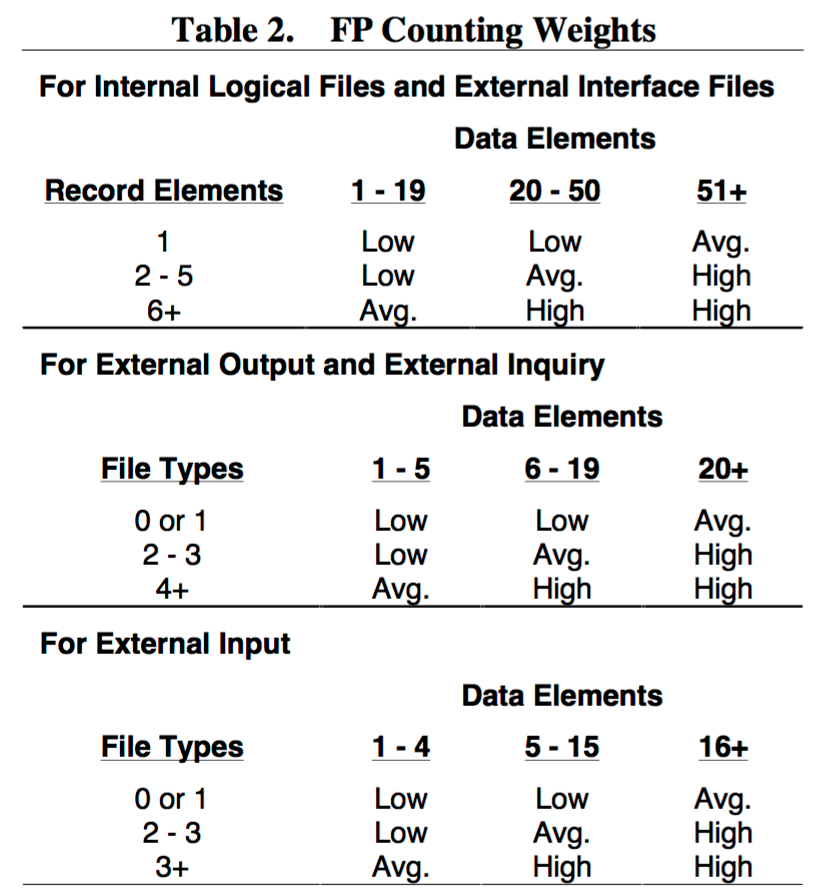
\includegraphics[keepaspectratio=true,scale=0.3]{Pictures/TableComplexity.png}}
%			\end{minipage}		
%			\bigskip\\
%			\smallskip\\
			The schema below defines the weights assigned to every level of complexity for all the FP types.\smallskip\\
			\begin{minipage}{\linewidth}
				%			\vspace*{-0.35cm}
				\makebox[\linewidth]{
					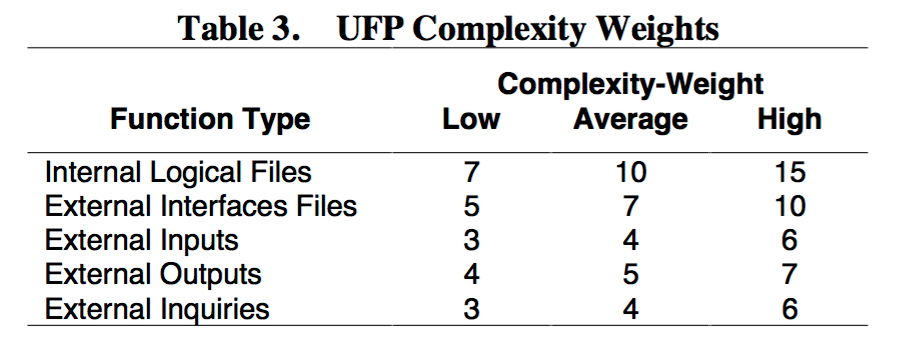
\includegraphics[keepaspectratio=true,scale=0.3]{Pictures/TableWeights.png}}
			\end{minipage}
			\bigskip\\
			Here is a brief explanation of the FP types:
			\begin{itemize}
				\item Internal Logic File: homogeneous set of data used and managed by the application
				\item External Interface File: homogeneous set of data used by the application but generated and maintained by other applications
				\item External Input: elementary operation to elaborate data coming from the external environment
				\item External Output: elementary operation that generates data for the external environment (it usually includes the elaboration of data from logic files)
				\item External Inquiry: Elementary operation that involves input and output (without significant elaboration of data from logic files)
				
			\end{itemize}
	
		\subsection{FP types estimation}
			The assignation of the complexity to each functionality is based on the number of fields and interactions with other components required to implement it. 
			\begin{itemize}
				\item ILF
							\renewcommand{\arraystretch}{1.2}
							\setlength{\tabcolsep}{12pt}
					\begin{center}
						\begin{tabular}{| p{7cm} | p{2.5cm} | p{2cm} |}\hline
							\textbf{Functionalities} & \multicolumn{1}{|c|}{\textbf{Complexity}} & \textbf{FP Count}\\\hline
							Users & \multicolumn{1}{|c|}{Simple} & \multicolumn{1}{|c|}{7}\\\hline
							Ride & \multicolumn{1}{|c|}{Complex} & \multicolumn{1}{|c|}{15}\\\hline
							Request & \multicolumn{1}{|c|}{Medium} & \multicolumn{1}{|c|}{10}\\\hline		
							Zone & \multicolumn{1}{|c|}{Medium} & \multicolumn{1}{|c|}{10}\\\hline	
							Taxi & \multicolumn{1}{|c|}{Simple} & \multicolumn{1}{|c|}{7}\\\hline		
							Payment-Receipts & \multicolumn{1}{|c|}{Simple} & \multicolumn{1}{|c|}{7}\\\hline																														
							\multicolumn{2}{|l|}{Total:} & \multicolumn{1}{|c|}{56}\\\hline
						\end{tabular}
					\end{center}
				\item EIF
				\renewcommand{\arraystretch}{1.2}
				\setlength{\tabcolsep}{12pt}
				\begin{center}
					\begin{tabular}{| p{7cm} | p{2.5cm} | p{2cm} |}\hline
						\textbf{Functionalities} & \multicolumn{1}{|c|}{\textbf{Complexity}} & \textbf{FP Count}\\\hline						
						Payment Data & \multicolumn{1}{|c|}{Medium} & \multicolumn{1}{|c|}{7}\\\hline
						Google Maps & \multicolumn{1}{|c|}{Medium} & \multicolumn{1}{|c|}{7}\\\hline
						Push notification metadata & \multicolumn{1}{|c|}{Simple} & \multicolumn{1}{|c|}{5}\\\hline		
						\multicolumn{2}{|l|}{Total:} & \multicolumn{1}{|c|}{19}\\\hline	
					\end{tabular}
				\end{center}
				\item Ext. INPUT
				\renewcommand{\arraystretch}{1.2}
				\setlength{\tabcolsep}{12pt}
				\begin{center}
					\begin{tabular}{| p{7cm} | p{2.5cm} | p{2cm} |}\hline
						\textbf{Functionalities} & \multicolumn{1}{|c|}{\textbf{Complexity}} & \textbf{FP Count}\\\hline
						Login & \multicolumn{1}{|c|}{Simple} & \multicolumn{1}{|c|}{3}\\\hline
						SignUp & \multicolumn{1}{|c|}{Simple} & \multicolumn{1}{|c|}{3}\\\hline
						Create request & \multicolumn{1}{|c|}{Simple} & \multicolumn{1}{|c|}{3}\\\hline					
						Pay & \multicolumn{1}{|c|}{Medium} & \multicolumn{1}{|c|}{4}\\\hline		
						Delete request & \multicolumn{1}{|c|}{Complex} & \multicolumn{1}{|c|}{6}\\\hline	
						Set taxi availability & \multicolumn{1}{|c|}{Simple} & \multicolumn{1}{|c|}{3}\\\hline					
						Accept/reject ride request & \multicolumn{1}{|c|}{Simple} & \multicolumn{1}{|c|}{3}\\\hline			
						Update taxi position & \multicolumn{1}{|c|}{Simple} & \multicolumn{1}{|c|}{3}\\\hline				
						Manage taxi drivers & \multicolumn{1}{|c|}{Medium} & \multicolumn{1}{|c|}{4}\\\hline				
						Create ride & \multicolumn{1}{|c|}{Complex} & \multicolumn{1}{|c|}{6}\\\hline		
						Allocate taxi & \multicolumn{1}{|c|}{Complex} & \multicolumn{1}{|c|}{6}\\\hline																																																												
						\multicolumn{2}{|l|}{Total:} & \multicolumn{1}{|c|}{44}\\\hline
					\end{tabular}
				\end{center}
				\item Ext. INQUIRY
				\renewcommand{\arraystretch}{1.2}
				\setlength{\tabcolsep}{12pt}
				\begin{center}
					\begin{tabular}{| p{7cm} | p{2.5cm} | p{2cm} |}\hline
						\textbf{Functionalities} & \multicolumn{1}{|c|}{\textbf{Complexity}} & \textbf{FP Count}\\\hline
						Request history & \multicolumn{1}{|c|}{Simple} & \multicolumn{1}{|c|}{3}\\\hline
						Manage profile & \multicolumn{1}{|c|}{Simple} & \multicolumn{1}{|c|}{3}\\\hline
						Ride history & \multicolumn{1}{|c|}{Simple} & \multicolumn{1}{|c|}{3}\\\hline		
						Public API & \multicolumn{1}{|c|}{Medium} & \multicolumn{1}{|c|}{4}\\\hline	
						DB & \multicolumn{1}{|c|}{Medium} & \multicolumn{1}{|c|}{4}\\\hline		

						\multicolumn{2}{|l|}{Total:} & \multicolumn{1}{|c|}{17}\\\hline
					\end{tabular}
				\end{center}
				\item Ext. OUTPUT
				\renewcommand{\arraystretch}{1.2}
				\setlength{\tabcolsep}{12pt}
				\begin{center}
					\begin{tabular}{| p{7cm} | p{2.5cm} | p{2cm} |}\hline
						\textbf{Functionalities} & \multicolumn{1}{|c|}{\textbf{Complexity}} & \textbf{FP Count}\\\hline
						SMS & \multicolumn{1}{|c|}{Simple} & \multicolumn{1}{|c|}{4}\\\hline
						Email & \multicolumn{1}{|c|}{Simple} & \multicolumn{1}{|c|}{4}\\\hline
						PushNotification & \multicolumn{1}{|c|}{Simple} & \multicolumn{1}{|c|}{4}\\\hline		
						Monitor Zone & \multicolumn{1}{|c|}{Medium} & \multicolumn{1}{|c|}{5}\\\hline																						
						\multicolumn{2}{|l|}{Total:} & \multicolumn{1}{|c|}{17}\\\hline
					\end{tabular}
				\end{center}
				\pagebreak
				\item Total and conclusions
				\renewcommand{\arraystretch}{1.2}
				\setlength{\tabcolsep}{12pt}
				\begin{center}
					\begin{tabular}{| p{7cm} | p{2cm} |}\hline
						\textbf{FP types} & \multicolumn{1}{|c|}{\textbf{Value}}\\\hline
						ILF & \multicolumn{1}{|c|}{56}\\\hline
						EIF & \multicolumn{1}{|c|}{19}\\\hline
						Ext. INPUT & \multicolumn{1}{|c|}{44}\\\hline
						Ext. INQUIRY & \multicolumn{1}{|c|}{17}\\\hline		
						Ext. OUTPUT & \multicolumn{1}{|c|}{17}\\\hline																						
						Total: & \multicolumn{1}{|c|}{153}\\\hline
					\end{tabular}
				\end{center}																					
			\end{itemize}
			\bigskip	
			The total number of FPs it then 153.\bigskip\\
			We can use this number to estimate the number of lines of code needed for the project; to do this a conversion factor is used: 46.\\
			This value is obtained from the average value for J2EE language from the table at\\ \href{http://www.qsm.com/resources/function-point-languages-table}{http://www.qsm.com/resources/function-point-languages-table.}\bigskip\\
			Thus the estimate of SLOC will be: \begin{center}\(153FPs * 46 = 7038 \ SLOC\)\end{center}
			This result is the starting point for the next evaluation technique, the COCOMO approach.
	\pagebreak		
	\section{COCOMO II analysis}
		\subsection{Introduction}	
			This estimation is achieved through a complex, statistical model that takes in account the characteristics of the product but also of people and process. The result of this technique is the estimation of Person-Months required to develop the project.\\
			The COCOMO II calculations are based on the estimated of the software dimension in source lines of code (SLOC).
			Two very important metrics are used for this evaluation:
			\begin{itemize}
				\item Scale Drivers: the 5 SD determine the exponent used in the ``effort equation''
				\item Cost Drivers: the 17 Cost Drivers represent the multiplicative factors that determine the effort required to complete the project
			\end{itemize}
			The result, the so-called ``\textit{Effort equation}'' is:
			\begin{center}\($\euro$ffort = 2.94 * EAF * (KSLOC)^E \ [Person$-$Months]\)\end{center}
			Where:
			\begin{itemize}
				\item \textit{EAF}: Effort Adjustment Factor derived from Cost Drivers (product of the effort multipliers corresponding to each of the cost drivers for the project)
				\item \textit{E}: Exponent derived from SD
				\item \textit{KSLOC}: SLOC measured in thousands
			\end{itemize}
			Once the effort has been computed it is possible to calculate the number of months required to complete the project with the duration equation:
			\begin{center}\(Duration = 3.67 * ($\euro$ffort)^E \ [Months]\)\end{center}
			Where:
			\begin{itemize}
				\item \textit{\euro ffort}: is the effort computed above
				\item \textit{E}: is the schedule equation exponent derived from the five Scale Drivers
			\end{itemize}	
			When both the \textit{\euro ffort} and the \textit{Duration} are available then the number of people required to complete the project is:
			\begin{center}\(N_{people} = \lceil $\euro$ / D \rceil \ [People]\)\end{center}
		\subsection{Parameters choice and estimation}
			A first estimation is carried out considering a project with all “nominal” Cost Drivers and Scale Drivers: this means an \textit{EAF} of 1.00 and exponent \textit{E} of 1.0997. The effort equation thus becomes: 
			\begin{center}\($\euro$ffort = 2.94 * 1.0 * (7.038)^{1.0997} = 25.13 \ Person$-$Months\)\end{center}
			Proceeding with the computation of the schedule equation the formula with the nominal parameter of \textit{E} = 0.3179 becomes:
			\begin{center}\(Duration = 3.67 * (25.13)^{0.3179} = 10.23 \ Months\)\end{center}
			The size of the team is then:
			\begin{center}\(N_{people} = \lceil 25.13 / 10.23 \rceil = \lceil 2.45 \rceil = 3 \ People\)\end{center}
			The analysis gives the following result: it takes about 10 months of 3 people-work to finish this project.
			\bigskip\\
		\subsection{Second analysis with automated tool}
			A second analysis is here presented; it has been done with the help of an online tool \linebreak \href{http://csse.usc.edu/tools/COCOMOII.php}{(http://csse.usc.edu/tools/COCOMOII.php)}, where it is easier and immediate to evaluate the difference in effort and scheduling as parameters of drivers change.\bigskip\\
			In particular the variations with respect to the nominal case are the following:
			\begin{itemize}
				\item Precedentedness: LOW, because the team has not much experience on large scale Java Enterprise projects with such high quality and reliability requirements
				\item Architecture/Risk Resolution: HIGH, since the team wants to avoid mistakes that can be raised during the development at a late stage that could involve the feasibility of the project itself; this is achieved through a thorough analysis of the architecture and the possible risks.
				\item Required Software Reliability: HIGH, since the expected quality of the system is very high, and on it depend a lot of processes (passenger clients, drivers, the public transportation for whole cities...)
			\end{itemize}\bigskip
			Below are the settings of this analysis.\bigskip\\
			\begin{minipage}{\linewidth}
				%			\vspace*{-0.35cm}
				\makebox[\linewidth]{
					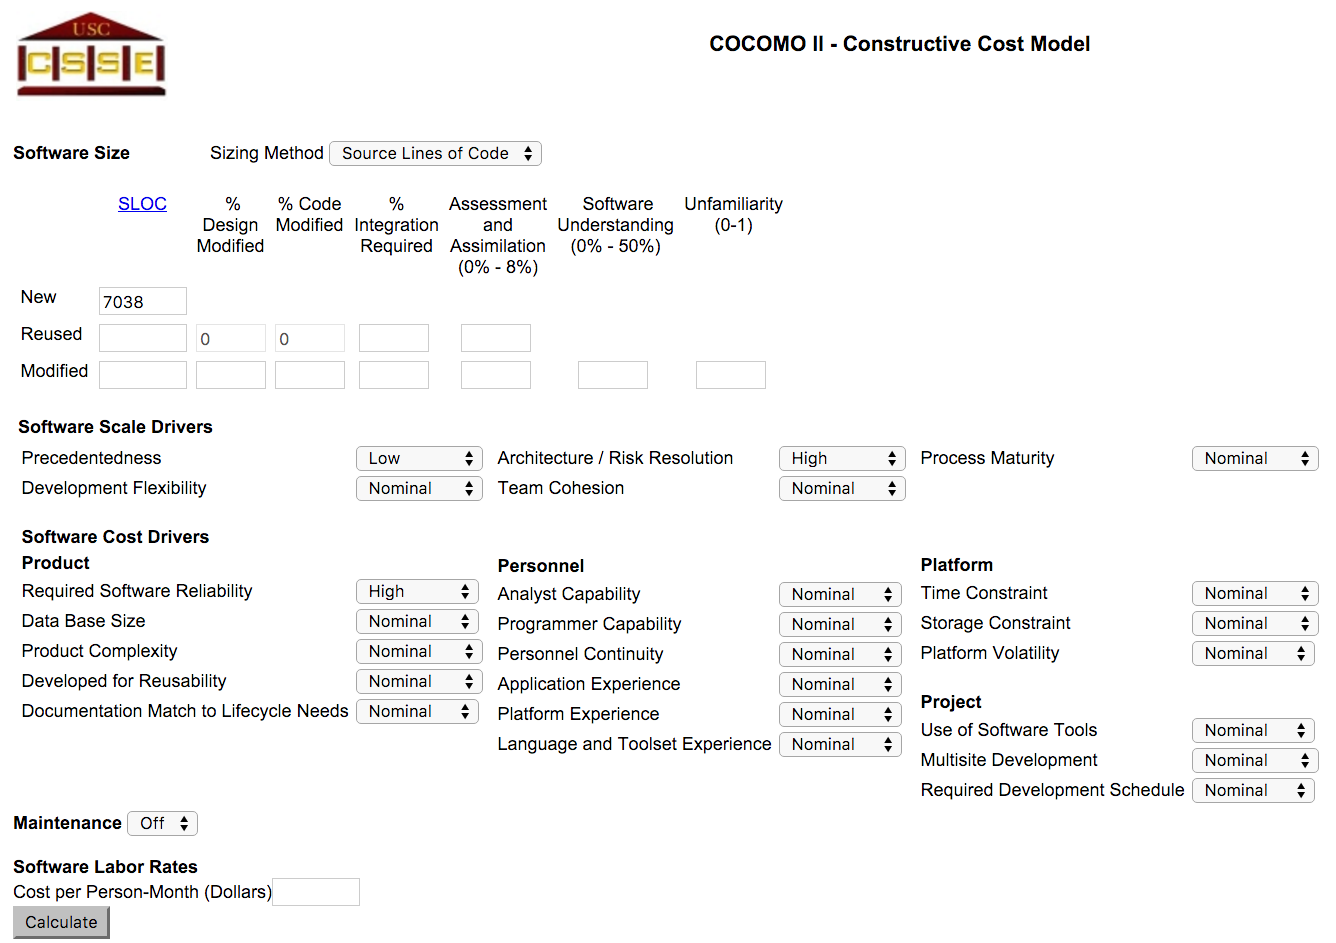
\includegraphics[keepaspectratio=true,scale=0.36]{Pictures/COCOMOparameters.png}}
			\end{minipage}
			\pagebreak\\
			Below is the output of the analysis.\bigskip\\
			\begin{minipage}{\linewidth}
				%			\vspace*{-0.35cm}
				\makebox[\linewidth]{
					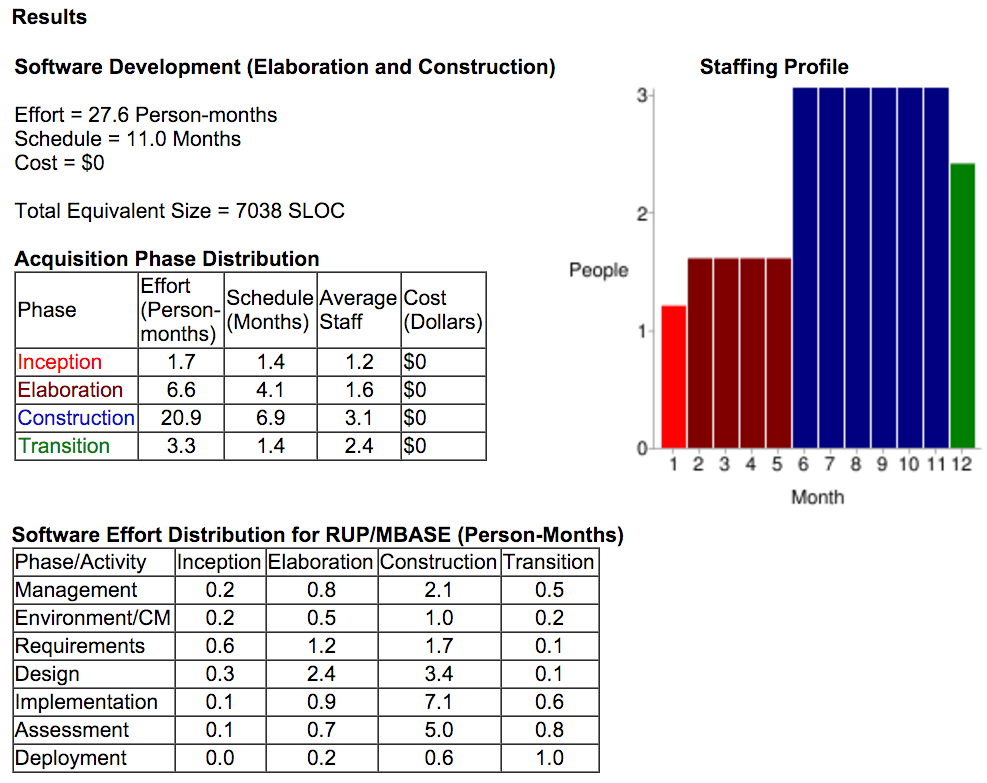
\includegraphics[keepaspectratio=true,scale=0.4]{Pictures/COCOMOoutput.png}}
			\end{minipage}
			\bigskip\\
			The slight variation due to the different parameters does not really change the estimation:
			\begin{itemize}
				\item Duration: from about 10 to 11 months.
				\item Size of the team: always 3 people required  (\(N_{people} = \lceil 27.6 / 11 \rceil = \lceil 2.5 \rceil = 3 \ People\))
			\end{itemize}
			\bigskip
			This obvious result is a direct consequence of the increase in risk control and high-quality-software objectives prefixed with the parameters.
			
	\pagebreak
	\section{Tasks identification}	
		The ``Waterfall Model'' of the software life-cycle is used as a guideline for the choice of the tasks and their order of execution.
		\renewcommand{\arraystretch}{1.2}
		\setlength{\tabcolsep}{7pt}
		\begin{center}
			\resizebox{0.9\textwidth}{!}{\begin{minipage}{\textwidth}
			\begin{tabular}{| c | c | c | c | c |}\hline
				\multicolumn{1}{|c|}{\textbf{ID}} & \multicolumn{1}{|c|}{\textbf{Task}} & {\textbf{Effort}} & \multicolumn{1}{|c|}{\textbf{Duration}} & \multicolumn{1}{|c|}{\textbf{Dependencies}}\\
				
				 &  & {\textbf{[Person-Days]}} & \multicolumn{1}{|c|}{\textbf{[Days]}} &\\\hline				
				
%				\textbf{ID} & \textbf{Task} & \parbox{3cm}{Effort \\  [Person-Days]} & \textbf{Duration [Days]} & \textbf{Dependencies}		
					
				\multicolumn{1}{|c|}{T1} & \multicolumn{1}{|c|}{Stakeholders identification} & \multicolumn{1}{|c|}{5} & \multicolumn{1}{|c|}{2} & \multicolumn{1}{|c|}{}\\\hline
				
				\multicolumn{1}{|c|}{T2} & \multicolumn{1}{|c|}{Actors identification} & \multicolumn{1}{|c|}{5} & \multicolumn{1}{|c|}{2} & \multicolumn{1}{|c|}{T1}\\\hline	
				
				\multicolumn{1}{|c|}{T3} & \multicolumn{1}{|c|}{Goals identification} & \multicolumn{1}{|c|}{12} & \multicolumn{1}{|c|}{4} & \multicolumn{1}{|c|}{T2}\\\hline							

				\multicolumn{1}{|c|}{T4} & \multicolumn{1}{|c|}{Requirements identification} & \multicolumn{1}{|c|}{18} & \multicolumn{1}{|c|}{6} & \multicolumn{1}{|c|}{T3}\\\hline
				
				\multicolumn{1}{|c|}{T5} & \multicolumn{1}{|c|}{Use Case and Scenarios} & \multicolumn{1}{|c|}{11} & \multicolumn{1}{|c|}{4} & \multicolumn{1}{|c|}{T4}\\\hline
				
				\multicolumn{1}{|c|}{T6} & \multicolumn{1}{|c|}{Class diagram} & \multicolumn{1}{|c|}{18} & \multicolumn{1}{|c|}{6} & \multicolumn{1}{|c|}{T5}\\\hline	
				
				\multicolumn{1}{|c|}{T7} & \multicolumn{1}{|c|}{Alloy model} & \multicolumn{1}{|c|}{10} & \multicolumn{1}{|c|}{5} & \multicolumn{1}{|c|}{T6}\\\hline	
				
				\multicolumn{1}{|c|}{T8} & \multicolumn{1}{|c|}{Components and interfaces} & \multicolumn{1}{|c|}{24} & \multicolumn{1}{|c|}{12} & \multicolumn{1}{|c|}{T7}\\\hline		
				
				\multicolumn{1}{|c|}{T9} & \multicolumn{1}{|c|}{Deployment architecture} & \multicolumn{1}{|c|}{17} & \multicolumn{1}{|c|}{9} & \multicolumn{1}{|c|}{T8}\\\hline			
				
				\multicolumn{1}{|c|}{T10} & \multicolumn{1}{|c|}{Runtime elements} & \multicolumn{1}{|c|}{15} & \multicolumn{1}{|c|}{8} & \multicolumn{1}{|c|}{T9}\\\hline			
				
				\multicolumn{1}{|c|}{T11} & \multicolumn{1}{|c|}{Algorithms design} & \multicolumn{1}{|c|}{28} & \multicolumn{1}{|c|}{10} & \multicolumn{1}{|c|}{T8}\\\hline	
				
				\multicolumn{1}{|c|}{T12} & \multicolumn{1}{|c|}{Sequence diagrams} & \multicolumn{1}{|c|}{19} & \multicolumn{1}{|c|}{7} & \multicolumn{1}{|c|}{T8}\\\hline				
		
				\multicolumn{1}{|c|}{T13} & \multicolumn{1}{|c|}{User interface mock-up} & \multicolumn{1}{|c|}{25} & \multicolumn{1}{|c|}{25} & \multicolumn{1}{|c|}{T5}\\\hline		
				
				\multicolumn{1}{|c|}{T14} & \multicolumn{1}{|c|}{Client manager development} & \multicolumn{1}{|c|}{30} & \multicolumn{1}{|c|}{15} & \multicolumn{1}{|c|}{T10, T11, T12, T13}\\\hline	
				
				\multicolumn{1}{|c|}{T15} & \multicolumn{1}{|c|}{Account manager development} & \multicolumn{1}{|c|}{32} & \multicolumn{1}{|c|}{16} & \multicolumn{1}{|c|}{T10, T11, T12}\\\hline
				
				\multicolumn{1}{|c|}{T16} & \multicolumn{1}{|c|}{Request manager development} & \multicolumn{1}{|c|}{65} & \multicolumn{1}{|c|}{22} & \multicolumn{1}{|c|}{T10, T11, T12}\\\hline		
				
				\multicolumn{1}{|c|}{T17} & \multicolumn{1}{|c|}{Ride manager development} & \multicolumn{1}{|c|}{38} & \multicolumn{1}{|c|}{19} & \multicolumn{1}{|c|}{T10, T11, T12}\\\hline	
				
				\multicolumn{1}{|c|}{T18} & \multicolumn{1}{|c|}{Zone manager development} & \multicolumn{1}{|c|}{73} & \multicolumn{1}{|c|}{25} & \multicolumn{1}{|c|}{T10, T11, T12}\\\hline	
				
				\multicolumn{1}{|c|}{T19} & \multicolumn{1}{|c|}{Taxi manager development} & \multicolumn{1}{|c|}{15} & \multicolumn{1}{|c|}{15} & \multicolumn{1}{|c|}{T10, T11, T12}\\\hline	
				
				\multicolumn{1}{|c|}{T20} & \multicolumn{1}{|c|}{Notification manager development} & \multicolumn{1}{|c|}{18} & \multicolumn{1}{|c|}{18} & \multicolumn{1}{|c|}{T10, T11, T12}\\\hline	
				
				\multicolumn{1}{|c|}{T21} & \multicolumn{1}{|c|}{Payment manager development} & \multicolumn{1}{|c|}{18} & \multicolumn{1}{|c|}{18} & \multicolumn{1}{|c|}{T10, T11, T12}\\\hline	
				
				\multicolumn{1}{|c|}{T22} & \multicolumn{1}{|c|}{Integration testing strategy} & \multicolumn{1}{|c|}{35} & \multicolumn{1}{|c|}{12} & \multicolumn{1}{|c|}{from T14 to T21}\\\hline	
				
				\multicolumn{1}{|c|}{T23} & \multicolumn{1}{|c|}{Integration testing execution} & \multicolumn{1}{|c|}{40} & \multicolumn{1}{|c|}{14} & \multicolumn{1}{|c|}{T22}\\\hline	
				
				\multicolumn{1}{|c|}{T24} & \multicolumn{1}{|c|}{Software deployment} & \multicolumn{1}{|c|}{10} & \multicolumn{1}{|c|}{4} & \multicolumn{1}{|c|}{T23}\\\hline	
			\end{tabular}
		\end{minipage} }
		\end{center}
		The effort measured in Person-Months can be converted in Person-Days taking into account that in a months there are about 21 working days, so the 27.6 Person-Months are equivalent to \(27.6 * 21 = 580 \ Person$-$Days \). The sum of the column ``Effort'' of the table above should match that figure.
	
	\section{Task scheduling and Resources allocation}	
		Below are shown the Gantt diagrams representing the guideline for the scheduling of the project which helps respecting the deadlines and deliverables.\\
		First is presented an overall view of the whole project, later on the focus is on the particular of every section of the project.\\
		Be aware that in the charts the US date format is used!\smallskip\\
		The meaning of the colors is:
		\begin{itemize}
			\item GREEN: all the 3 members of the team are working on the task
			\item ORANGE: two member of the project are working on the task
			\item PURPLE: just one member of the group is working on that task.
		\end{itemize}
		\begin{minipage}{\linewidth}
			%			\vspace*{-0.35cm}
			\makebox[\linewidth]{
				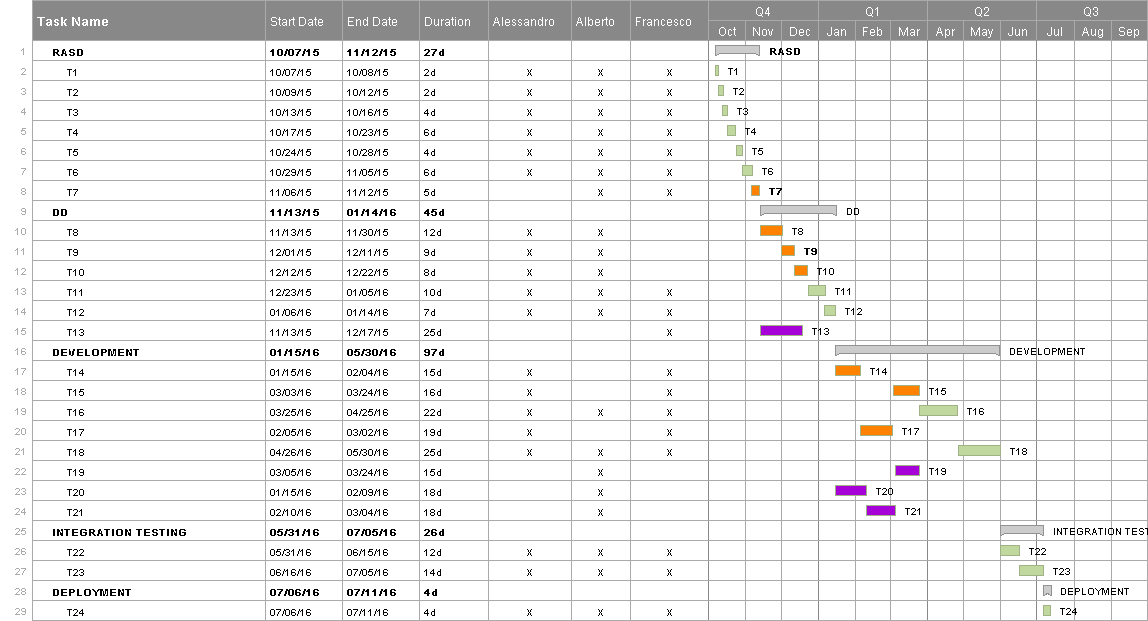
\includegraphics[keepaspectratio=true,scale=0.6,angle=90,origin=c]{Pictures/PlanOverall.png}}
		\end{minipage}			
		\begin{center}
			Scheduling and resources allocation for RASD document
		\end{center}		
		\begin{minipage}{\linewidth}
			%			\vspace*{-0.35cm}
			\makebox[\linewidth]{
				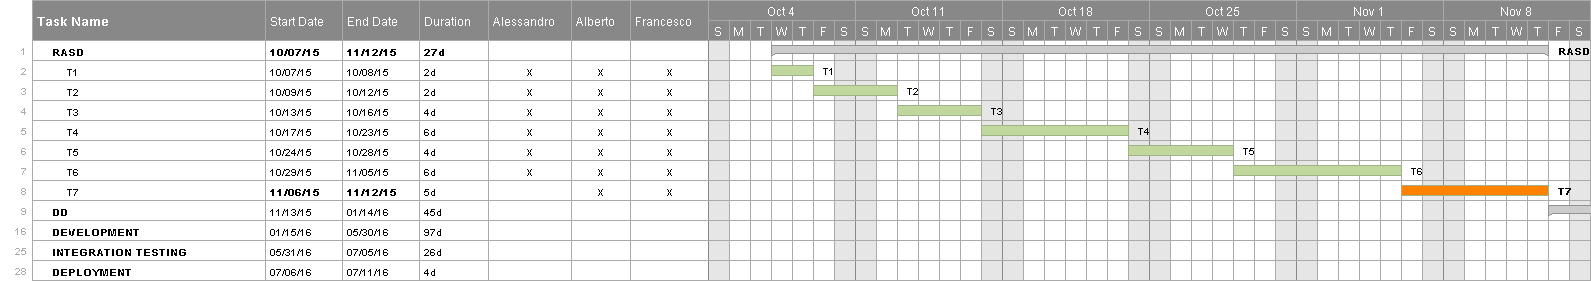
\includegraphics[keepaspectratio=true,scale=0.43,angle=90,origin=c]{Pictures/PlanRASD.png}}
		\end{minipage}
		\begin{center}
			Scheduling and resources allocation for Design document
		\end{center}
		\begin{minipage}{\linewidth}
			%			\vspace*{-0.35cm}
			\makebox[\linewidth]{
				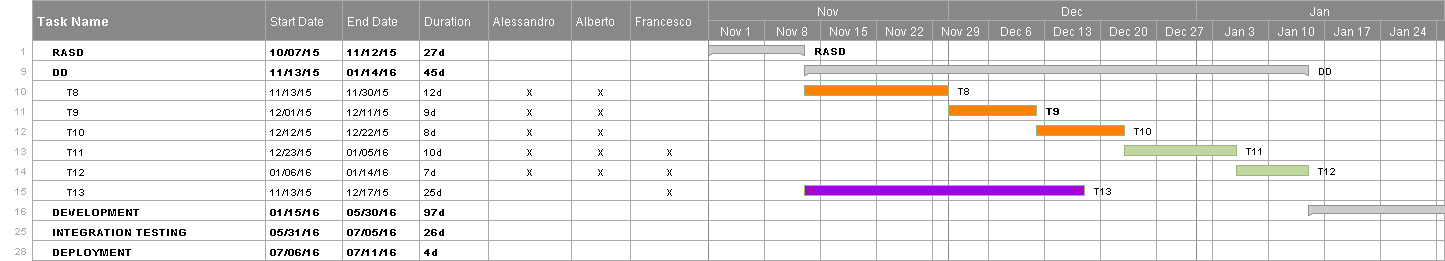
\includegraphics[keepaspectratio=true,scale=0.47,angle=90,origin=c]{Pictures/PlanDD.png}}
		\end{minipage}		
		\begin{center}
			Scheduling and resources allocation for the development phase
		\end{center}
		\begin{minipage}{\linewidth}
			%			\vspace*{-0.35cm}
			\makebox[\linewidth]{
				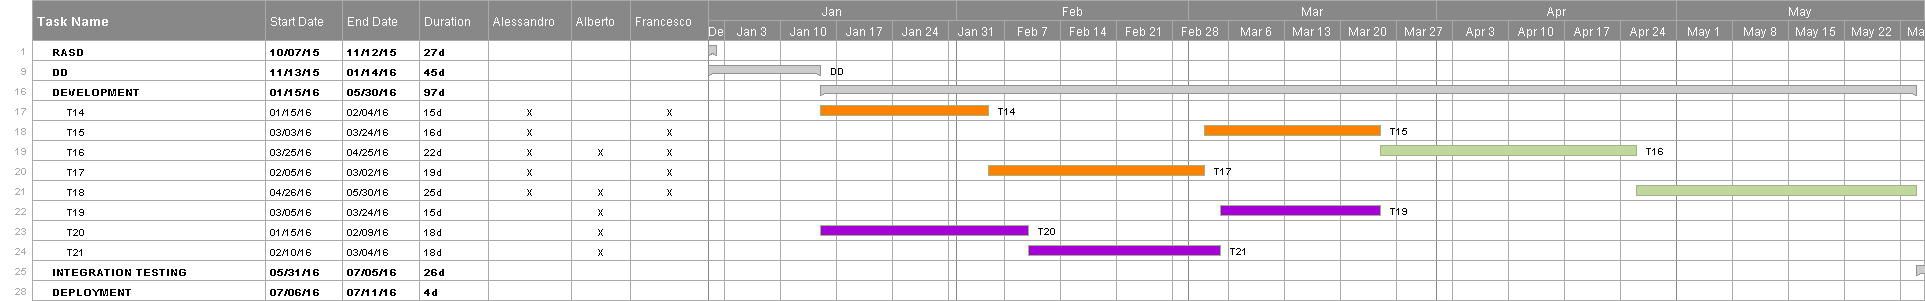
\includegraphics[keepaspectratio=true,scale=0.355,angle=90,origin=c]{Pictures/PlanDevelopment.png}}
		\end{minipage}	
		\begin{center}
			Scheduling and resources allocation for integration testing
		\end{center}		
		\begin{minipage}{\linewidth}
			%			\vspace*{-0.35cm}
			\makebox[\linewidth]{
				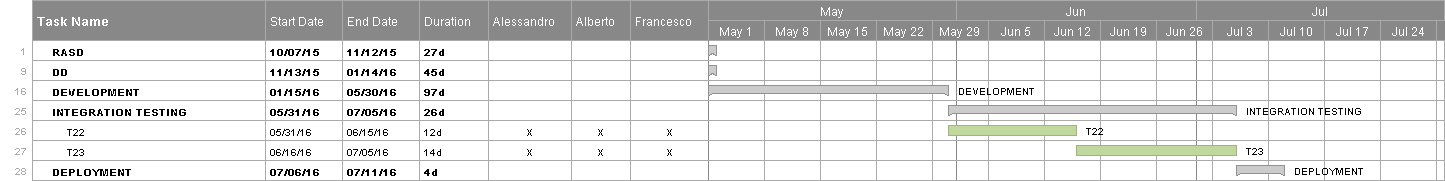
\includegraphics[keepaspectratio=true,scale=0.47,angle=90,origin=c]{Pictures/PlanIntegration.png}}
		\end{minipage}	
		\begin{center}
			Scheduling and resources allocation for deployment of the final product
		\end{center}	
		\begin{minipage}{\linewidth}
			%			\vspace*{-0.35cm}
			\makebox[\linewidth]{
				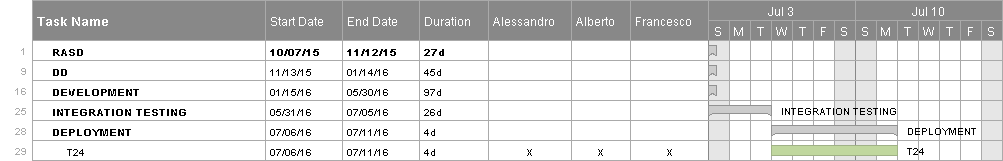
\includegraphics[keepaspectratio=true,scale=0.67,angle=90,origin=c]{Pictures/PlanDeployment.png}}
		\end{minipage}
		The following diagram shows the allocation of the three people in the team in a more clear way, with the tasks grouped by person.\\
		\begin{minipage}{\linewidth}
			%			\vspace*{-0.35cm}
			\makebox[\linewidth]{
				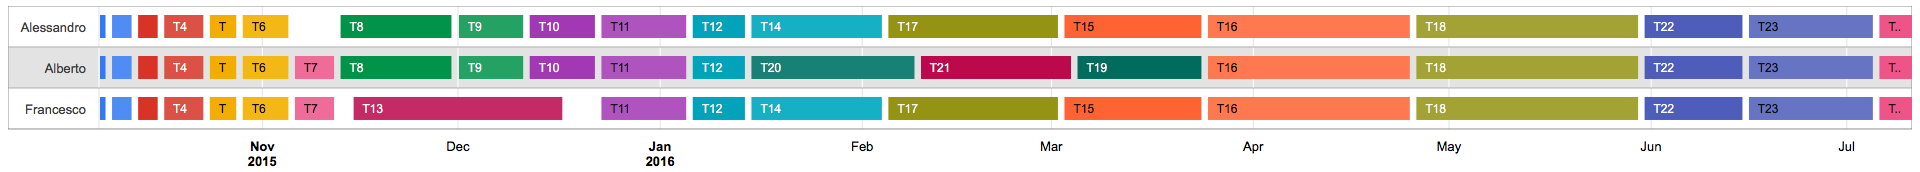
\includegraphics[keepaspectratio=true,scale=0.35,angle=90,origin=c]{Pictures/ResourcesAllocation.png}}
		\end{minipage}
		It is important to notice that in the scheduling of the project and in the allocation of resources the difference between business days and weekends has been taken into account. The workweek is from Monday to Friday, while the weekend is Saturday and Sunday. Days are 8 hours of work time.\\
		For instance the tasks T1 and T2 are both 2-day long, but the latter covers the weekend, so it has been counted up for 4 days instead of 2.\bigskip\\
		Federal holidays have not been considered since this is an approximate schedule, but they could cause up to about 10 days of delay on the proposed schedule.\\
		\smallskip\\
		The proposed schedule matches the 10/11 months expected duration of the project forecast with the COCOMO analysis, in fact the planned work starts October 7, 2015 and ends July 11, 2016.
	
	\pagebreak
	\vspace*{-1.3cm}
	\section{Risk planning and management}
		The main factors of risk are related to project and technical ones; after an analysis of all the possible risks, those which are ranked higher in the probability-of-occurrence list are:
		\begin{enumerate}
			\item Unrealistic schedule
			\item Availability of staff
			\item Wrong functionalities
			\item Wrong User Interface
			\item Bad external components
			\item Real-time shortfalls
		\end{enumerate}	
		A \textit{proactive} strategy is employed, thus a contingency plan is developed to handle unavoidable risks in a controlled and effective manner.\bigskip\\
		Respectively:
		\begin{enumerate}
			\item To avoid delays in the scheduled work, the work plan itself has been drafted with more relaxed time windows for every deadline, taking into account a possible lower pace of work and effort to foresee such problems.
			\item This strategy also covers the possibility of delays due to illness of key staff at critical times: being the due-date of the sections stretched a bit more, the other components of the team are able to catch up with the work of the unavailable members. Besides many tasks are carried out together, with the allocation of all the three co-workers, to bypass the overhead time that would be lost when a member has to complete a task not assigned to himself to cover an unavailable colleague. In other situations two members of the team work on high priority and complex tasks, while the third person carries on another task in parallel. Being the task assigned to the single individual simpler (e.g. User Interface mock-ups), if it happens that he is ill, the others can easily continue its work.
			\item Many interviews with stakeholders and other managers of the project are organized as soon as the project is assigned to the team. It is in the interest of both the parties (stakeholders and developing team) to correctly understand the target functionalities of the system to-be-produced. Besides often \textit{milestones} are scheduled to be screened with the client, so as to have a constant check on the goals and functionalities that can be assessed and possibly corrected at any moment, in order to avoid sudden changes in requirements that require a major design rework.
			\item Mock-ups of the final GUI are drafted at an early stage; these are sent to the client for approval and possibly corrected. During the screening of milestones the client is able to test the GUI and the interactions with the system in order to have a continual assessment of these.
			\item The external components on which the team relies to set-up the system (e.g. payment provider, SMS and email services) are high quality ones offered by well known companies that have been in the business for years. This choice has been taken to avoid dependencies with just-created unknown services which could be unreliable or shut-down in the near future. Others are bought-in components of known reliability, easily replaceable.
			\item In order to offer an high quality service and fast response-time of the system, the whole service has been calibrated to handle many more connections and higher work-load than the real estimate of future use. All the components have been ``underestimated'' and tested in the worst conditions of usage.
		\end{enumerate}		

	\pagebreak
	\section{References}
		Material from Wikipedia
		\begin{itemize}
			\item Project management: \href{https://en.wikipedia.org/wiki/Project\_management\#Planning}{https://en.wikipedia.org/wiki/Project\_management\#Planning}
		\end{itemize}
	
	\section{Appendix}
		\subsection{Software and tools used}
		\begin{itemize}
			\item TeXstudio 2.10.6 (\href{http://www.texstudio.org/}{http://www.texstudio.org/}) to redact and format this document.
			\item Astah Professional 7.0 (\href{http://astah.net/editions/professional}{http://astah.net/editions/professional}) 
		\end{itemize}
		
		\subsection{Hours of work} The time spent to redact this document:
		\begin{itemize}
			\item Baldassari Alessandro: 12 hours.
			\item Bendin Alberto: 12 hours.
			\item Giarola Francesco: 12 hours.
		\end{itemize}

\end{document}